%% =============================================================================
\section*{Performance Analysis}
%% =============================================================================

This section analyses the timing data collected across the performance tests in the previous section. 
All timings exclude timed-out rows (20\,s limit) when computing averages.

%% =============================================================================
\subsubsection*{Build Time Analysis Across Verification Modes}
%% =============================================================================

Figure~\ref{fig:build-time-modes-m3} plots average build times for each
configuration across the three verification modes.

\begin{figure}[H]
\centering
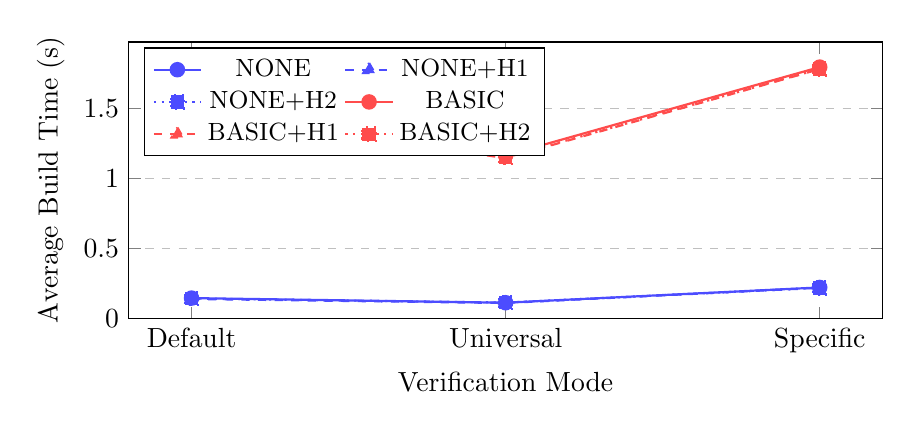
\begin{tikzpicture}
\begin{axis}[
    width=0.92\linewidth,
    height=0.42\linewidth,
    xlabel={Verification Mode},
    ylabel={Average Build Time (s)},
    symbolic x coords={Default,Universal,Specific},
    xtick=data,
    legend style={at={(0.02,0.98)}, anchor=north west, font=\small, legend columns=2},
    ymajorgrids=true,
    grid style=dashed,
    ymin=0,
    mark options={scale=1.2}
]
% NONE family
\addplot[color=blue!70, mark=*, thick] coordinates {
    (Default,0.145) (Universal,0.112) (Specific,0.221)
};
\addlegendentry{NONE}

\addplot[color=blue!70, mark=triangle*, thick, dashed] coordinates {
    (Default,0.139) (Universal,0.110) (Specific,0.219)
};
\addlegendentry{NONE+H1}

\addplot[color=blue!70, mark=square*, thick, dotted] coordinates {
    (Default,0.142) (Universal,0.113) (Specific,0.218)
};
\addlegendentry{NONE+H2}

% BASIC family
\addplot[color=red!70, mark=*, thick] coordinates {
    (Default,1.452) (Universal,1.163) (Specific,1.793)
};
\addlegendentry{BASIC}

\addplot[color=red!70, mark=triangle*, thick, dashed] coordinates {
    (Default,1.482) (Universal,1.143) (Specific,1.779)
};
\addlegendentry{BASIC+H1}

\addplot[color=red!70, mark=square*, thick, dotted] coordinates {
    (Default,1.481) (Universal,1.147) (Specific,1.780)
};
\addlegendentry{BASIC+H2}

\end{axis}
\end{tikzpicture}
\caption{Average build time per configuration across verification modes.
Blue lines = NONE family (no loop optimisation); red lines = BASIC family
(with loop-collapse).  Hints do not materially affect build time.}
\label{fig:build-time-modes-m3}
\end{figure}

The NONE family stays flat and cheap across all modes ($0.11$--$0.22$\,s), because
the CHC system is built with no additional pre-processing.
BASIC-family configurations pay a fixed overhead of roughly $1.1$--$1.8$\,s for
the loop-collapse pass; this cost is mode-independent, rising only with program size.
Within BASIC, Specific mode is the most expensive ($1.79$\,s) because its
programs carry additional symbolic parameters that expand the loop-collapse
computation.  Hints have negligible effect on build time in both families.

%% =============================================================================
\subsubsection*{Solve Time Analysis Across Verification Modes}
%% =============================================================================

Figure~\ref{fig:solve-time-modes-m3} plots average solve times (excluding timeouts).

\begin{figure}[H]
\centering
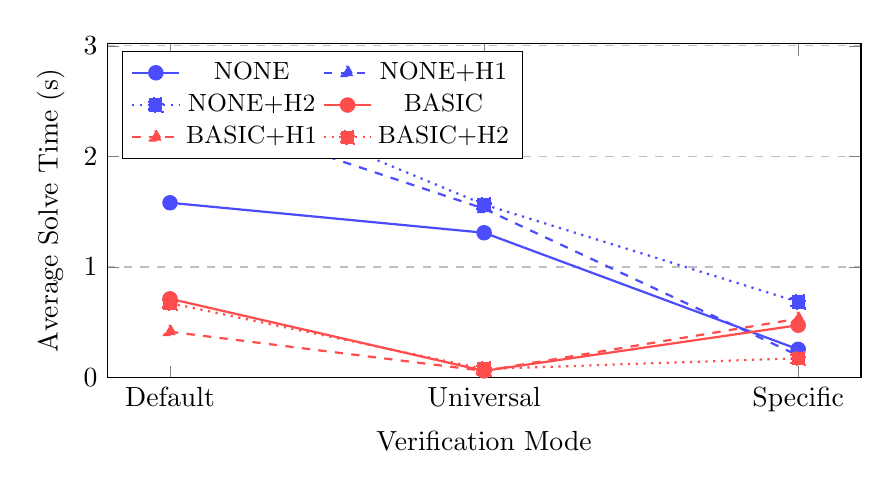
\begin{tikzpicture}
\begin{axis}[
    width=0.92\linewidth,
    height=0.48\linewidth,
    xlabel={Verification Mode},
    ylabel={Average Solve Time (s)},
    symbolic x coords={Default,Universal,Specific},
    xtick=data,
    legend style={at={(0.02,0.98)}, anchor=north west, font=\small, legend columns=2},
    ymajorgrids=true,
    grid style=dashed,
    ymin=0,
    mark options={scale=1.2}
]
% NONE family
\addplot[color=blue!70, mark=*, thick] coordinates {
    (Default,1.581) (Universal,1.310) (Specific,0.256)
};
\addlegendentry{NONE}

\addplot[color=blue!70, mark=triangle*, thick, dashed] coordinates {
    (Default,2.473) (Universal,1.527) (Specific,0.200)
};
\addlegendentry{NONE+H1}

\addplot[color=blue!70, mark=square*, thick, dotted] coordinates {
    (Default,2.743) (Universal,1.565) (Specific,0.685)
};
\addlegendentry{NONE+H2}

% BASIC family
\addplot[color=red!70, mark=*, thick] coordinates {
    (Default,0.713) (Universal,0.061) (Specific,0.474)
};
\addlegendentry{BASIC}

\addplot[color=red!70, mark=triangle*, thick, dashed] coordinates {
    (Default,0.415) (Universal,0.061) (Specific,0.533)
};
\addlegendentry{BASIC+H1}

\addplot[color=red!70, mark=square*, thick, dotted] coordinates {
    (Default,0.674) (Universal,0.078) (Specific,0.175)
};
\addlegendentry{BASIC+H2}

\end{axis}
\end{tikzpicture}
\caption{Average solve time per configuration (timeouts excluded from average).
H2 (\texttt{heading\_on\_grid\_always}) can \emph{raise} solve time under NONE
because the added assumption enlarges the CHC formula without the structural
simplification that BASIC provides.}
\label{fig:solve-time-modes-m3}
\end{figure}

The key contrast is between NONE and BASIC is, BASIC reduces the number of CHC rules
seen by Spacer, so the solver's \emph{per-query} time drops dramatically,
especially for Universal mode (from $\approx 1.3$\,s down to $0.06$\,s).
For NONE-family configurations, H2 increases average solve time in Default mode
($1.58 \to 2.74$\,s) because injecting the heading constraint adds a large
disjunctive guard to every rule, and without loop-collapse Spacer must reason
over many more rule instances.  Under BASIC the situation reverses: the collapsed
loop already carries the grid invariant so H2's guard is cheap to discharge,
dropping Specific solve time from $0.47$ to $0.18$\,s.

%% =============================================================================
\subsubsection*{Timeout and Optimisation Benefits}
%% =============================================================================

\paragraph{Verdict distribution.}
Figure~\ref{fig:verdict-stacked-m3} shows the distribution of outcomes
(proved/UNSAT, counterexample found/SAT, timeout) for all six configurations
across the three modes.

\begin{figure}[H]
\centering
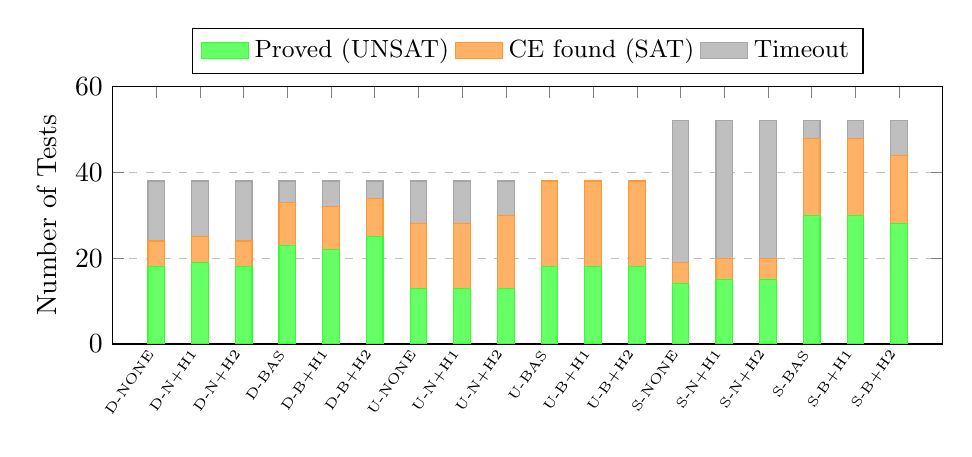
\begin{tikzpicture}
\begin{axis}[
    ybar stacked,
    width=\linewidth,
    height=0.40\linewidth,
    bar width=6pt,
    ymajorgrids=true,
    grid style=dashed,
    ylabel={Number of Tests},
    xtick={1,2,3,4,5,6,7,8,9,10,11,12,13,14,15,16,17,18},
    xticklabels={
        D-NONE, D-N+H1, D-N+H2, D-BAS, D-B+H1, D-B+H2,
        U-NONE, U-N+H1, U-N+H2, U-BAS, U-B+H1, U-B+H2,
        S-NONE, S-N+H1, S-N+H2, S-BAS, S-B+H1, S-B+H2
    },
    x tick label style={rotate=55, anchor=east, font=\tiny},
    xmin=0, xmax=19,
    legend style={at={(0.5,1.05)}, anchor=south, legend columns=3, font=\small},
    ymin=0, ymax=60,
    area legend
]

% Proved (UNSAT) - green
\addplot[fill=green!60, draw=green!80] coordinates {
    (1,18) (2,19) (3,18) (4,23) (5,22) (6,25)
    (7,13) (8,13) (9,13) (10,18) (11,18) (12,18)
    (13,14) (14,15) (15,15) (16,30) (17,30) (18,28)
};
\addlegendentry{Proved (UNSAT)}

% CE found (SAT) - orange
\addplot[fill=orange!60, draw=orange!80] coordinates {
    (1,6) (2,6) (3,6) (4,10) (5,10) (6,9)
    (7,15) (8,15) (9,17) (10,20) (11,20) (12,20)
    (13,5) (14,5) (15,5) (16,18) (17,18) (18,16)
};
\addlegendentry{CE found (SAT)}

% Timeout - gray
\addplot[fill=gray!50, draw=gray!70] coordinates {
    (1,14) (2,13) (3,14) (4,5) (5,6) (6,4)
    (7,10) (8,10) (9,8) (10,0) (11,0) (12,0)
    (13,33) (14,32) (15,32) (16,4) (17,4) (18,8)
};
\addlegendentry{Timeout}

\end{axis}
\end{tikzpicture}
\caption{Verdict distribution across all modes (D=Default, U=Universal, S=Specific)
and configurations (N=NONE, BAS=BASIC).  Green = invariant proved; orange = expected
counterexample found; gray = solver timed out.}
\label{fig:verdict-stacked-m3}
\end{figure}

\paragraph{Incremental benefit of the loop-collapse optimisation (BASIC).}
Table~\ref{tab:basic-gain-m3} shows how many previously-timed-out tests become
solvable when NONE is upgraded to BASIC, and how many (if any) regress.

\begin{table}[H]
\centering
\caption{Tests rescued from timeout by the BASIC loop-collapse optimisation
(NONE $\to$ BASIC).  Regressions are tests that timed out under BASIC but not under NONE.}
\label{tab:basic-gain-m3}
\begin{tabular}{lccc}
\toprule
\textbf{Mode} & \textbf{Rescued} & \textbf{Regressions} & \textbf{Net gain} \\
\midrule
Default   & 13 & 4 & +9 \\
Universal & 10 & 0 & +10 \\
Specific  & 31 & 2 & +29 \\
\midrule
\textbf{Total} & \textbf{54} & \textbf{6} & \textbf{+48} \\
\bottomrule
\end{tabular}
\end{table}

\paragraph{Milestone~2 vs.\ Milestone~3 comparison.}
Table~\ref{tab:m2-m3-compare} compares test completion rates between Milestone~2
and Milestone~3.  Despite the three-fold reduction
in time budget, M3 solves substantially more tests in every mode and configuration.

\begin{table}[H]
\centering
\caption{Test completion rates: Milestone~2 (20\,s timeout) vs.\ Milestone~3 (20\,s timeout).}
\label{tab:m2-m3-compare}
\begin{tabular}{lcccccc}
\toprule
& \multicolumn{2}{c}{\textbf{Default (38 tests)}}
& \multicolumn{2}{c}{\textbf{Universal (38 tests)}}
& \multicolumn{2}{c}{\textbf{Specific (52 tests)}} \\
\cmidrule(lr){2-3}\cmidrule(lr){4-5}\cmidrule(lr){6-7}
\textbf{Config} & \textbf{M2} & \textbf{M3} & \textbf{M2} & \textbf{M3} & \textbf{M2} & \textbf{M3} \\
\midrule
NONE       & 39\% & 63\% & 68\% &  74\% & 25\% & 37\% \\
BASIC      & 58\% & 87\% & 89\% & 100\% & 35\% & 92\% \\
BASIC+hint & 61\% & 89\% & 92\% & 100\% & 37\% & 92\% \\
\bottomrule
\end{tabular}
\end{table}

The biggest improvement is in specific mode: \textit{\texttt{Milestone-2}} \texttt{BASIC} solved only 18 of 52 tests
($35\%$), while \textit{\texttt{Milestone-3}} \texttt{BASIC} solves 48 of 52 ($92\%$).
The improvement comes from the loop-collapse encoding,
which transforms deep parametric loops (e.g.\ \texttt{s\_repeat\_100},
\texttt{s\_nest\_4}, \texttt{s\_wide}) into compact fixed-point systems that
\textsc{Spacer} closes in under $0.2$\,s.

A secondary improvement is build time for Universal-mode trigonometric programs:
\textit{\texttt{Milestone-2}} \texttt{BASIC} built \texttt{perf\_trig\_10} and related programs in $190$--$210$\,s each
due to symbolic expansion of \texttt{repeat}/\texttt{forward} loops; M3 BASIC
handles the same programs in $\approx 1.7$\,s (a $\approx 120\times$ reduction).
In exchange, \textit{\texttt{Milestone-3}} \texttt{BASIC} spends $3$--$9\times$ more build time than M2 on simple loop
programs (e.g.\ \texttt{repeat\_10}) because the new pass performs a deeper algebraic
analysis.

\paragraph{Hint benefits (H1 and H2).}
Table~\ref{tab:hint-gain-m3} shows the number of timeouts eliminated by each hint
independently and the number of tests that \emph{regressed} (a previously-passing
configuration now times out) under the assumption hint H2.

\begin{table}[H]
\centering
\caption{Timeout reduction by hints relative to the no-hint baseline.
``Rescued'' = timeout$\to$solved; ``Regressions'' = solved$\to$timeout.}
\label{tab:hint-gain-m3}
\begin{tabular}{llcc}
\toprule
\textbf{Transition} & \textbf{Mode} & \textbf{Rescued} & \textbf{Regressions} \\
\midrule
NONE $\to$ NONE+H1   & Default   & 1 & 0 \\
                      & Universal & 0 & 0 \\
                      & Specific  & 1 & 0 \\
\midrule
NONE $\to$ NONE+H2   & Default   & 0 & 0 \\
                      & Universal & 2 & 0 \\
                      & Specific  & 1 & 0 \\
\midrule
BASIC $\to$ BASIC+H1 & Default   & 0 & 1 \\
                      & Universal & 0 & 0 \\
                      & Specific  & 0 & 0 \\
\midrule
BASIC $\to$ BASIC+H2 & Default   & 3 & 2 \\
                      & Universal & 0 & 0 \\
                      & Specific  & 0 & 4 \\
\bottomrule
\end{tabular}
\end{table}

\paragraph{Representative rescued tests.}
Table~\ref{tab:rescued-examples-m3} lists specific program--property pairs that
time out under the baseline and are rescued by a particular configuration.
These cases demonstrate that the choice of optimisation and hint is
\emph{necessary}.

\begin{table}[H]
\centering
\small
\caption{Specific tests that time out ($\geq20$\,s) under the baseline and are
rescued by the indicated configuration.  Solve time shown is for the rescuing
configuration.}
\label{tab:rescued-examples-m3}
\begin{tabular}{llllr}
\toprule
\textbf{Program} & \textbf{Property} & \textbf{Mode} & \textbf{Rescuing config} & \textbf{Solve (s)} \\
\midrule
\multicolumn{5}{l}{\textit{Tight upper bounds --- require BASIC loop-collapse}} \\
\midrule
\texttt{repeat\_100}  & $x \leq 100$         & Default   & BASIC      & 0.034 \\
\texttt{repeat\_50}   & $x \leq 50$          & Default   & BASIC      & 0.052 \\
\texttt{deep\_nest\_3}& $c \leq 64$          & Default   & BASIC      & 0.069 \\
\texttt{deep\_nest\_4}& $d \leq 81$          & Default   & BASIC      & 0.078 \\
\texttt{many\_branches}& $x \leq 6$          & Default   & BASIC      & 0.092 \\
\texttt{wide\_vars}   & $a \leq 6$           & Default   & BASIC      & 0.078 \\
\texttt{s\_repeat\_100}& $x \leq 100$        & Specific  & BASIC      & 0.080 \\
\texttt{s\_nest\_4}   & $d \leq 256$         & Specific  & BASIC      & 0.150 \\
\texttt{s\_wide}      & $a \leq 6$           & Specific  & BASIC      & 0.067 \\
\midrule
\multicolumn{5}{l}{\textit{Heading-grid properties --- require BASIC+H2}} \\
\midrule
\texttt{turns\_20}    & heading on 24-grid   & Default   & BASIC+H2   & 0.079 \\
\texttt{turns\_20}    & heading $\in\{0,345\}$ & Default & BASIC+H2   & 0.318 \\
\texttt{turns\_50}    & heading $\in\{0,345\}$ & Default & BASIC+H2   & 0.287 \\
\midrule
\multicolumn{5}{l}{\textit{Property complexity --- require NONE+H1}} \\
\midrule
\texttt{repeat\_10}   & 11-way exact disj.   & Default   & NONE+H1    & 19.756 \\
\bottomrule
\end{tabular}
\end{table}


%% =============================================================================
\subsubsection*{Overall Performance}
%% =============================================================================

% Figure~\ref{fig:overall-completion-m3} summarises completion rates across all
% 128 tests for each configuration.  BASIC (no hints) achieves the highest overall
% rate (93.0\%), with the hint variants slightly below due to isolated regressions.

% \begin{figure}[H]
% \centering
% \begin{tikzpicture}
% \begin{axis}[
%     ybar,
%     width=0.88\linewidth,
%     height=0.44\linewidth,
%     bar width=14pt,
%     ymajorgrids=true,
%     grid style=dashed,
%     xlabel={Configuration},
%     ylabel={Overall Completion Rate (\%)},
%     xtick={1,2,3,4,5,6},
%     xticklabels={NONE, NONE+H1, NONE+H2, BASIC, BASIC+H1, BASIC+H2},
%     x tick label style={rotate=30, anchor=east, font=\small},
%     xmin=0, xmax=7,
%     ymin=0, ymax=100,
%     nodes near coords,
%     nodes near coords align={vertical},
%     every node near coord/.append style={font=\small},
% ]

% \addplot[fill=blue!40, draw=black] coordinates {
%     (1,55.5) (2,57.0) (3,57.8) (4,93.0) (5,92.2) (6,90.6)
% };

% \end{axis}
% \end{tikzpicture}
% \caption{Overall test completion rates across all 128 benchmark tests.
% \texttt{BASIC} (no hints) achieves the highest completion at 93.0\%.
% Hint variants trade minor regressions for small gains in specific scenarios.}
% \label{fig:overall-completion-m3}
% \end{figure}

Figure~\ref{fig:completion-by-mode-m3} breaks completion rate down per mode,
allowing comparison across the three verification settings.

\begin{figure}[H]
\centering
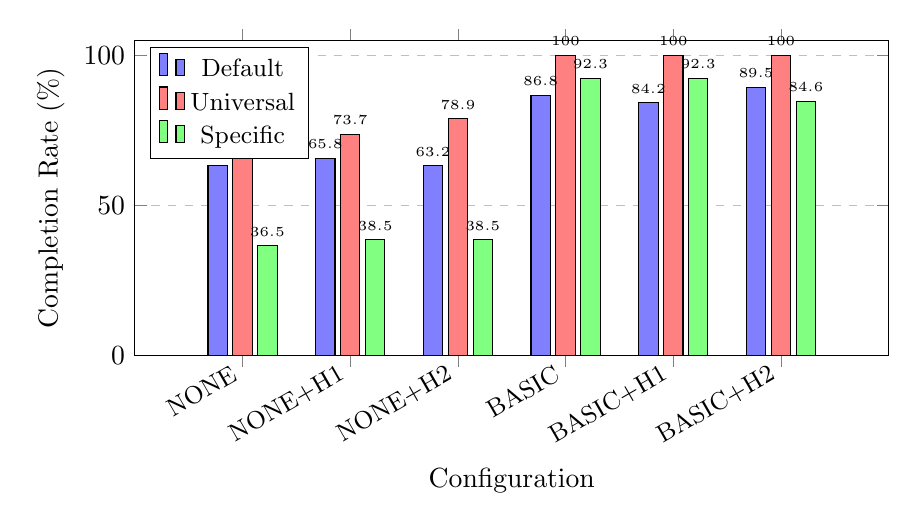
\begin{tikzpicture}
\begin{axis}[
    ybar,
    width=0.92\linewidth,
    height=0.46\linewidth,
    bar width=7pt,
    ymajorgrids=true,
    grid style=dashed,
    xlabel={Configuration},
    ylabel={Completion Rate (\%)},
    xtick={1,2,3,4,5,6},
    xticklabels={NONE, NONE+H1, NONE+H2, BASIC, BASIC+H1, BASIC+H2},
    x tick label style={rotate=30, anchor=east, font=\small},
    xmin=0, xmax=7,
    ymin=0, ymax=105,
    legend style={at={(0.02,0.98)}, anchor=north west, font=\small},
    nodes near coords,
    nodes near coords align={vertical},
    every node near coord/.append style={font=\tiny},
]

\addplot[fill=blue!50, draw=black] coordinates {
    (1,63.2) (2,65.8) (3,63.2) (4,86.8) (5,84.2) (6,89.5)
};
\addlegendentry{Default}

\addplot[fill=red!50, draw=black] coordinates {
    (1,73.7) (2,73.7) (3,78.9) (4,100.0) (5,100.0) (6,100.0)
};
\addlegendentry{Universal}

\addplot[fill=green!50, draw=black] coordinates {
    (1,36.5) (2,38.5) (3,38.5) (4,92.3) (5,92.3) (6,84.6)
};
\addlegendentry{Specific}

\end{axis}
\end{tikzpicture}
\caption{Completion rates broken down by verification mode.  Universal mode reaches
100\% under all BASIC variants.  Specific mode is most sensitive to hint choice:
H2 introduces regressions under BASIC.}
\label{fig:completion-by-mode-m3}
\end{figure}

%% =============================================================================
\subsubsection*{When to Use Each Configuration}
%% =============================================================================

\begin{itemize}[leftmargin=1.5em]

    \item \textbf{Prefer \texttt{BASIC} over \texttt{NONE}.}
    The M3 loop-collapse optimisation rescues 48 net tests from timeout compared to NONE,
    and raises the overall completion rate from $55\%$ to $93\%$.
    The only cost is a fixed build overhead ($\approx 1.1$--$1.8$\,s) that is negligible.

    \item \textbf{Add \texttt{H1} for trig-heavy programs with heading constraints.}
    H1 (\texttt{check\_heading\_always\_on\_grid})
    provides a moderate benefit for programs that turn on a 15-degree grid by adding a lightweight query-time constraint that
    helps Spacer close the heading-invariant without extra CHC rules.

    \item \textbf{Use \texttt{H2} under \texttt{BASIC}.}
    H2 (\texttt{heading\_on\_grid\_always}) is an \emph{assumption} hint: it
    strengthens the initial state, which is only sound if the program genuinely
    keeps heading on the grid throughout.  Under \texttt{NONE}, it enlarges every
    CHC rule with a disjunctive guard, worsening solve time.  Under
    \texttt{BASIC}, it rescues 3 Default tests and reduces Specific solve time
    from $0.47$ to $0.18$\,s.

   \item \textbf{Tight-bound properties benefit most from \texttt{BASIC}.}
    Properties such as $x \leq N$ (exact upper bound) and deep nesting invariants
    require Spacer to discover non-trivial loop invariants.  Under \texttt{NONE},
    every such test times out; under \texttt{BASIC}, the collapsed loop exposes the
    invariant structure directly to Spacer, reducing solve time from timeout to
    $< 0.1$\,s.

\end{itemize}
